\documentclass[10pt,conference]{resources/IEEEtran}

%%% Start Preamble
\usepackage[T1]{fontenc}
\usepackage[utf8]{inputenc}
\usepackage[english]{babel}
\AtBeginDocument{%
	\providecommand\BibTeX{{%
			\normalfont B\kern-0.5em{\scshape i\kern-0.25em b}\kern-0.8em\TeX}}}

\usepackage{hyperref}
\usepackage{cite}

\usepackage{amsmath,amssymb,amsfonts} %amsmath already included
\usepackage[noend]{algpseudocode}
\usepackage{algorithmicx, algorithm}
\usepackage{graphicx} %graphicx already included
\usepackage{textcomp}
\usepackage{xcolor}

\usepackage{tikz}
\usetikzlibrary{arrows,decorations.markings, positioning}
% \usepackage{subcaption}
\usepackage{tabu}

\hyphenation{con-straints}
%\pagestyle{plain}

%% COMMANDS:
\usepackage{resources/mathcommands}

%% DRAW SCHEDULES:
\usepackage{resources/scheduling}

%% THEOREMS:
% Theorems --
\usepackage{amsthm}
\usepackage{thmtools,thm-restate}

\newtheorem{theorem}{Theorem}%[section]
% \newtheorem{prop}[thm]{Proposition}
\newtheorem{lemma}[theorem]{Lemma}
\newtheorem{corollary}[theorem]{Corollary}
% \newtheorem{obs}[thm]{Observation}

\theoremstyle{definition}
\newtheorem{definition}[theorem]{Definition}
% \newtheorem{notn}[thm]{Notation}

% \declaretheorem[sibling=lemma,name=Lemma]{repeatablelemma}

% \theoremstyle{remark}
% \newtheorem{rmk}[thm]{Remark}
% \newtheorem{exmpl}[thm]{Example}

%\newtheorem{prog}[theorem]{Programming}
% \newtheorem{prog}{Programming}

% \newtheorem{corollary}{Corollary}
% --


%% WRITING:
\newcommand{\comment}[3]{{\color{#1}#2:#3}\ClassWarning{}{There are comments left in the paper. [Remove them before submission!]}}
\newcommand{\mario}[1]{\comment{red}{mg}{#1}}
\newcommand{\kuan}[1]{\comment{blue}{kh}{#1}}
\newcommand{\jj}[1]{\comment{orange}{jj}{#1}}

% \usepackage{lineno}
\usepackage[switch]{lineno}
\linenumbers
% fix problem with line numbering around align
\makeatletter
\let\LN@align\align
\let\LN@endalign\endalign
\renewcommand{\align}{\linenomath\LN@align}
\renewcommand{\endalign}{\LN@endalign\endlinenomath}
\makeatother


%% PAPER SPECIFIC:
\usetikzlibrary{patterns}
\ifCLASSOPTIONcompsoc
	\usepackage[caption=false,font=normalsize,labelfont=sf,textfont=sf]{subfig}
\else
	\usepackage[caption=false,font=footnotesize]{subfig}
\fi
\usepackage{enumitem}

\newcommand{\mrt}{\mathrm{MRT}}
\newcommand{\lat}{\mathrm{Lat}}

\newcommand{\fc}{\fw{c}}
\newcommand{\bc}{\bw{c}}
\newcommand{\pc}{{pc}}

\newcommand{\Tmaxone}{T^E_{\mathit{max},1}}
\newcommand{\Tmaxtwo}{T^E_{\mathit{max},2}}





%%% End Preamble




\begin{document}
	%% TITLE:
	\title{Optimal Task Phasing for End-To-End Latency in Harmonic Systems and Semi-Harmonic Automotive Systems}
	
	%% AUTHORS: Mario, Matthias
	
%	% Final version
%	\author{
%		\IEEEauthorblockN{First Author, Second Author and Third Author}
%		\IEEEauthorblockA{TU Dortmund University\\
%			Email: \{first.author, second.author, third.author\}@tu-dortmund.de}
%		\and
%		\IEEEauthorblockN{Other Author}
%		\IEEEauthorblockA{Other University\\
%			Email: other.author@other-university.de}
%		}
	
%	% Submission version:
	\author{RTAS 2025 Submission \# \textcolor{red}{TBD} \quad\quad\quad Pages: \pageref{last-page}}
	
	\maketitle
	\thispagestyle{plain}
	\pagestyle{plain}

	\begin{abstract}
		% - introductory sentence to the topic (optional)
		In the context of automotive systems, the end-to-end latency of a sequence of tasks (a so-called cause-effect chains) is a common metric to ensure correct timing behavior.
		% - describe the issue or main problem (create a need)
		To control the end-to-end latency, proper task configuration is crucial. 
		While the literature considers the configuration of task periods, optimization of task phases to minimize the end-to-end latency is only sparsely discussed. 

		% - one sentence detailing your approach (meet the need)
		In this work, we discuss the configuration of task phases to optimize the end-to-end latency of a cause-effect chain.
		% - list main research results
		To that end, we develop a strategy for semi-harmonic task systems, which are very common in industrial applications.
		% - finish with MAIN MESSAGE of the paper
		We prove that our strategy is optimal in the sense that it minimizes the end-to-end latency.
		Furthermore, our evaluation based on a real-world application shows that optimizing task phases can reduce end-to-end latencies significantly. 

		\mario{11 pages of technical content + bib and ackn; Track 2}
	\end{abstract} 
	
%	\vspace{-.2in}
	
	\section{Introduction}
	\label{sec:introduction}
	% General introduction

	% Topic of this paper
	
	% Detailed topic / tell more details


	State of the art: Release all tasks at the same time


	- Related work: Alessandro ECRTS

	\mario{This is the first work that exploits partitioned job chains analytically after their initial exploration in \cite{DBLP:conf/ecrts/GunzelTCBC23}.}


	\mario{TODO:
	- We use task set and task system interchangably, and say the task set/task system/system is harmonic. We need to make the language consistent.
	}
	
	
	% Contribution
	\noindent\textbf{Contributions:} % short text
	\begin{itemize}
		\item one
		\item two
		\item three
	\end{itemize}
	
\section{System Model}
\label{sec:system_model}

	In embedded systems, several tasks are deployed that each fulfills a different dedicated purpose.
	The set of all tasks is denoted as $\Tbb$.
	%
	To allow the embedded system to fulfill complex assignments, tasks have to interact with each other. 
	That is achieved by data exchange between tasks. 

	\smallskip
	\textbf{Task Model:}
	Each task $\tau\in \Tbb$ can be described by a tuple $(C_\tau, T_\tau, \phi_\tau) \in \Rbb^3$.
	More specifically, $C_\tau >0$ is the worst-case execution time (WCET) of $\tau$, $T_\tau > 0$ is the task period, and $\phi_\tau$ is the task phase.
	The task recurrently releases jobs, denoted by $\tau(m),~m\in \Nbb {=} \setof{0,1,2,\dots}$ according to its description.
	That is, $\tau(0)$ is released at time $\phi_\tau$, and subsequent jobs are released every $T_{\tau}$ time units, i.e., $\tau(m)$ is released at time $\phi_\tau + m \cdot T_{\tau}$. 
	Each job $\tau(m)$ executes for at most $C_\tau$ time units.
	We consider implicit-deadline tasks where the deadline of each job is at the release of the subsequent job, i.e., the deadline of $\tau(m)$ is at $\phi_\tau + (m+1) T_{\tau}$.

	Task systems are \emph{harmonic} if all task periods are integer multiples of one another.
	That is, for any two tasks $\tau, \tau' \in \Tbb$, we have 
	\begin{equation}
		\frac{T_{\tau}}{T_{\tau'}} \in \Nbb \qquad \text{or} \qquad \frac{T_{\tau'}}{T_{\tau}} \in \Nbb.
	\end{equation}
	Harmonic task systems have the benefit that their release pattern is highly repetitive. As a result, the data propagation through these tasks is easier to analyze and to control.
	For the results of this work, weaker forms of harmonic are already sufficient.
	Specifically, in Section~\ref{sec:harmonic}, we consider \emph{max-harmonic} subsets $\Tbb' \subseteq \Tbb$, where 
	\begin{equation}
		\frac{\max_{\tau\in \Tbb'} T_{\tau}}{T_{\tau}} \in \Nbb
	\end{equation}
	for all $\tau \in \Tbb'$. 
	For the results in Section~\ref{sec:automotive}, we consider semi-harmonic task sets $\Tbb$ with 
	\begin{equation}
		T_\tau \in \setof{1,2,5,10,20,50,100,200,1000}
	\end{equation}
	for all $\tau \in \Tbb$.
	These semi-harmonic task sets are common in the automotive domain~\cite{kramer2015real}.

	\smallskip
	\textbf{Task communication:}
	To transmit data between tasks, they need to communicate. 
	We assume that the communication can be modeled via shared resources. 
	That is, a task writes data to a shared resource (overwriting previous data), and the successor tasks reads the data from that shared resource. 
	In this work, we focus on the communication model of the Logical Execution Time (LET)~\cite{DBLP:conf/birthday/KirschS12} mechanism, where each job reads data at its release and writes data at its deadline.
	More specifically, the read-event of $\tau(m)$ is at time 
	\begin{equation}
		\re (\tau(m)) := \phi_{\tau} + m \cdot T_{\tau},
	\end{equation}
	and the write-event of $\tau(m)$ is at time 
	\begin{equation}
		\we (\tau(m)) := \phi_{\tau} + (m+1) \cdot T_{\tau}.
	\end{equation}
	We assume that communication overheads are negligible, which is realized by existing LET implementations~\cite{Biondi2018LET, Bellassai2023JSA7}.
	
	\smallskip
	\textbf{Scheduling Model:}
	The results of this work are versatile in the sense that we do not rely on a specific scheduling model.
	For example, typical Fixed-Priority (FP) schedulers like Rate-Monotonic (RM) and Deadline-Monotonic (DM), or Dynamic-Priority (DP) schedulers like Earliest-Deadline-First (EDF) can be applied. 
	To ensure that task communication via LET can be realized, schedulability of the task system needs to be verified. 
	This can be done using appropriate schedulability tests for the underlying scheduling model.


\section{Cause-Effect Chains and End-to-End latencies}
\label{sec:e2e}

	To achieve complex functionalities, usually several tasks have to cooperate. 
	A sequence of cooperating tasks is called a cause-effect chain 
	\begin{equation}
		E=(\tau_1 \to \dots \to \tau_n)
	\end{equation}
	with $n\in \Nbb_{\geq 1}$.
	Specifically, data that is written by $\tau_i$ is read by $\tau_{i+1}$, for $i=1, \dots, n-1$.
	The underlying functionality is achieved when data has been propagated through all $n$ tasks. 
	For this work, we denote by 
	\begin{equation}
		\Tbb_E := \setof{\tau_1, \dots, \tau_n} \subseteq \Tbb
	\end{equation}
	the tasks of $\Tbb$ that are part of the cause-effect chain.
	Furthermore, we assume that $\tau_i \neq \tau_j$ for all $i \neq j$.

	\mario{I think we need a simple application-oriented example with a picture here.}

	In the literature, two metrics for the end-to-end latency are usually considered:
	\begin{enumerate}
		\item Maximum Reaction Time: \emph{How long does it take until an external activity is processed?}
		\item Maximum Data Age: \emph{How old is data used in an actuation?}
	\end{enumerate}
	Recently, it was shown that both metrics are equivalent~\cite{DBLP:conf/ecrts/GunzelTCBC23}.
	Therefore, we do not distinguish those metrics and use the term \emph{end-to-end latency} ($\lat(E)$) universally.
	Further, it was shown in~\cite{DBLP:conf/ecrts/GunzelTCBC23} that \emph{partitioned job chains} can be used to define the end-to-end latency.
	Partitioned job chains rely on immediate forward and immediate backward job chains~\cite{duerrCASES}, which are used to track data propagation and data origin through the system, respectively.

	\begin{definition}[Immediate forward job chain]
		Let $m\in \Nbb$ and $E=(\tau_1\to \dots \to \tau_n)$ a cause-effect chain.
		The $m$-th \emph{immediate forward job chain} of $E$ is a sequence of jobs 
		\begin{math}
			\fc_m = (\tau_1(j_1) \to \dots \to \tau_n(j_n))
		\end{math}
		such that $j_1 = m$, and for all $i=1,\dots, n{-}1$ the job $\tau_{i+1}(j_{i+1})$ is the \emph{earliest} job of $\tau_{i+1}$ that reads data after it is written by $\tau_{i}(j_i)$, i.e., 
		\begin{math}
			j_{i+1} = \min \set{\xi \in \Nbb}{
			\we(\tau_i(j_i)) \leq 
			\re(\tau_{i+1}(\xi))
			}
			= \min \set{\xi \in \Nbb}{
			\phi_{\tau_i} + (j_i +1) \cdot T_{\tau_i} \leq 
			\phi_{\tau_{i+1}} + \xi \cdot T_{\tau_{i+1}}}.
		\end{math}
	\end{definition}

	\begin{definition}[Immediate backward job chain]
		Let $m\in \Nbb$ and $E=(\tau_1\to \dots \to \tau_n)$ a cause-effect chain.
		The $m$-th \emph{immediate backward job chain} of $E$ is a sequence of jobs 
		\begin{math}
			\bc_m = (\tau_1(j_1) \to \dots \to \tau_n(j_n))
		\end{math}
		such that $j_n = m$, and for all $i=2,\dots, n$ the job $\tau_{i-1}(j_{i-1})$ is the \emph{latest} job of $\tau_{i-1}$ that writes data before it is read by $\tau_{i}(j_i)$, i.e., 
		\begin{math}
			j_{i-1} 
			= \max \set{\xi \in \Nbb}{ 
			\we(\tau_{i-1}(\xi)) \leq \re(\tau_i(j_i))	
			}
			= \max \set{\xi \in \Nbb}{ \phi_{\tau_{i-1}} + (\xi+1) \cdot T_{\tau_{i-1}} \leq \phi_{\tau_i} + j_i \cdot T_{\tau_{i}}}.
		\end{math}
	\end{definition}

	We note that for some small $m$ the immediate backward job chain may not always exist in case $\set{\xi \in \Nbb}{ 
		\we(\tau_{i-1}(\xi)) \leq \re(\tau_i(j_i))	
		} = \emptyset$.
	Intuitively, this means that the job $\tau_{i}(j_i)$ has no data to process because task $\tau_{i-1}$ has not been executed yet.
	Such a scenario can only occur during the initial startup of the system.
	However, typical analyses are more interested in the system behavior during runtime when the system is already properly warmed up.
	We follow~\cite{DBLP:conf/ecrts/GunzelTCBC23} to determine the warm-up phase of each job.

	\begin{definition}[Warm-up]
		Consider the cause-effect chain $E=(\tau_1\to \dots \to \tau_n)$.
		Let $W_i\in \Nbb$, such that $\bc_W = (\tau_1(W_1) \to \dots \to \tau_n(W_n) )$ is the \emph{first} immediate backward job chain that exists. 
		We say that task $\tau_i$ is \emph{warmed up} with respect to $E$ at job $\tau_i(W_i)$.
	\end{definition}

	Intuitively, a task is warmed up with the first job that generates data that propagates to the end of the cause-effect chain without being overwritten.
	%
	In the following, we introduce partitioned job chains and properly define the end-to-end latency of $E$.

	\begin{definition}[Partitioned job chain.]
		Let $m\in \Nbb$, $E = (\tau_1\to\dots\to\tau_n)$, and  $p\in \setof{1, \dots, n}$.
		The $m$-th $p$-partitioned job chain of $E$ is a tuple
		\begin{equation}
			\pc^p_m = (\bc_m,\fc_{m+1})
		\end{equation}
		of an immediate backward and an immediate forward job chain.
		More specifically, $\bc_m$ is the $m$-th immediate backward job chain of $(\tau_1 \to \dots \to \tau_p)$, 
		and $\fc_{m+1}$ is the $(m+1)$-th immediate forward job chain of $(\tau_p \to \dots \to \tau_n)$.
	\end{definition}

	We note that the $\pc^p_m = (\bc_m,\fc_{m+1})$ exists if and only if its first entry $\bc_m$ exists.
	Hence, the $\pc^p_m$ exists for all $m\geq W_p$.
	%
	The length of $\pc^p_m = (\bc_m, \fc_{m+1})$ with $\bc_m = (\tau_1(j_1) \to\dots\to \tau_p(j_p))$ and $\fc_{m+1} = (\tau_p(j'_p) \to\dots\to \tau_n(j'_n))$ is defined as 
	\begin{align}
		\ell(\pc^p_m) 
		&:= 
		\we(\tau_n(j'_n)) - \re(\tau_1(j_1))
		\\&=
		(j'_n +1) \cdot T_{\tau_n} + \phi_{\tau_n} - (j_1 \cdot T_{\tau_1} + \phi_{\tau_1}).
	\end{align}
	% i.e., the distance between reading of the first job $\tau_1(j_1)$ and writing of the last job $\tau_n(j'_n)$.
	An example of a partitioned job chain is shown in Fig.~\ref{fig:chainExamples}.
	
	\begin{figure}
		\centering
		\footnotesize
		\begin{tikzpicture}[yscale=0.22, xscale=0.21]

			\begin{scope}[shift={(0,6)}] % task one
				\taskname{$\tau_1$}
				
				\timeline{0}{39}{}
				% no labelling
				
				% \releases{0,5,10}
				% \deadlines{5,10}
				
				\exec{0}{6}
				\exec[fill=red]{6}{12}
				\exec{12}{18}
				\exec{18}{24}
				\exec{24}{30}
				\exec{30}{36}
				\execopen{36}{38.5}
				
				% no suspension
			\end{scope}
			
			\begin{scope}[shift={(0,4.5)}] % task two
				\taskname{$\tau_2$}
				
				\timeline{0}{39}{}
				% \labelling{0}{13}{2}{0}
				
				% \releases{0}
				% \deadlines{12}
				
				\exec[pattern={north east lines}]{3}{7}
				\exec{7}{11}
				\exec{11}{15}
				\exec[fill=red]{15}{19}
				\exec[fill=blue]{19}{23}
				\exec{23}{27}
				\exec{27}{31}
				\exec{31}{35}
				\execopen{35}{38.5}

			\end{scope}

			\begin{scope}[shift={(0,3)}] % task three
				\taskname{$\tau_3$}
				
				\timeline{0}{39}{}
				% \labelling{0}{13}{2}{0}
				
				% \releases{0}
				% \deadlines{12}
				
				\exec[pattern={north east lines}]{0}{6}
				\exec[pattern={north east lines}]{6}{12}
				\exec{12}{18}
				\exec{18}{24}
				\exec[fill=blue]{24}{30}
				\exec{30}{36}
				\execopen{36}{38.5}

			\end{scope}

			\begin{scope}[shift={(0,1.5)}] % task four
				\taskname{$\tau_4$}
				
				\timeline{0}{39}{}
				\labelling{0}{39}{4}{0}
				
				% \releases{0}
				% \deadlines{12}
				
				\exec[pattern={north east lines}]{1}{5}
				\exec[pattern={north east lines}]{5}{9}
				\exec[pattern={north east lines}]{9}{13}
				\exec[pattern={north east lines}]{13}{17}
				\exec[pattern={north east lines}]{17}{21}
				\exec{21}{25}
				\exec{25}{29}
				\exec{29}{33}
				\exec[fill=blue]{33}{37}
				\execopen{37}{38.5}

			\end{scope}
		\end{tikzpicture}	
		\caption{A cause-effect chain $E=(\tau_1\rightarrow\tau_2\rightarrow\tau_3\rightarrow\tau_4)$ with LET communication semantics.  
			The partitioned job chain $\pc^2_4 = (\bc_4,\fc_5)$ is colorized. 
			The warm-up phase is indicated by jobs with hatched filling.} 
		\label{fig:chainExamples}
	\end{figure}

	\begin{definition}[End-to-end latency]
		The end-to-end latency of a cause-effect chain $E =(\tau_1\to\dots\to \tau_n)$ is the maximal length of $p$-partitioned job chains after the warm-up for any $p \in \setof{1, \dots, n}$.
		That is, 
		\begin{equation}
			\lat(E) = \sup_{m\geq W_p} \ell(\pc^p_m).
		\end{equation}		
	\end{definition}

	It is shown in~\cite{DBLP:conf/ecrts/GunzelTCBC23} that the end-to-end latency is independent of the choice of $p$, i.e., any $p \in \setof{1,\dots, n}$ can be chosen.

	Furthermore, for periodic tasks under LET, the read- and write-events repeat every hyperperiod $\lcm(T_{\tau_1}, \dots, T_{\tau_n})$ of $\Tbb_E$.
	Therefore, the partitioned job chains repeat every hyperperiod and only finitely many partitioned job chains need to be considered for the computation of the end-to-end latency. 
	
	\begin{restatable}{lemma}{lemmarepetetive}\label{lem:repetitive}
		Let $\mu(p) := \frac{H}{T_{\tau_p}}$ be the number of periods of $\tau_p$ that fit into one hyperperiod $H:= \lcm(T_{\tau_1}, \dots, T_{\tau_n})$ of $\Tbb_E$.
		We have
		\begin{equation}
			\ell(\pc^p_{m}) 
			= \ell\left(\pc^p_{m+\mu(p)}\right)
		\end{equation}
		for all $m \geq W_p$.
		In particular,  
		\begin{equation}
			\lat(E) = \max\left( \ell\left(\pc^p_{W_p}\right), \dots, \ell\left(\pc^p_{W_p+\mu(p)-1}\right) \right)
		\end{equation}
		holds.
	\end{restatable}

	While it is easy to convince ourselves that this lemma holds, the proof requires technical details and is moved to the \hyperref[sec:appendix]{Appendix} for readability. 





\section{Motivating Example}
\label{sec:motivation}

	In this section, we demonstrate the impact of task phasing on the end-to-end latency. 
	To that end, we consider an example cause-effect chain $E = (\tau_1 \to \tau_2 \to \tau_3)$ with: 
	\begin{equation}
		T_{\tau_1} = 10, \qquad T_{\tau_2}=1, \qquad T_{\tau_3}=10
	\end{equation}
	% \begin{itemize}
	% 	\item $T_1 = 10$
	% 	\item $T_2 = 1$
	% 	\item $T_3 = 10$
	% \end{itemize}
	%
	The typical approach of making the task set synchronous, i.e., 
	\begin{equation}
		\phi_{\tau_1} = \phi_{\tau_2} = \phi_{\tau_3} = 0 
	\end{equation}
	% $\tau_1, \tau_2, \tau_3 \in \mathit{Phase}(0)$ 
	leads to the schedule depicted in Figure~\ref{fig:motivation:synchronous}.
	%
	\begin{figure}
		\centering
		\subfloat[Synchronous: $\lat(E) = 40$.]{
		\footnotesize
		\begin{tikzpicture}[yscale=0.22, xscale=0.2]

			\begin{scope}[shift={(0,6)}] % task one
				\taskname{$\tau_1$}
				
				\timeline{0}{41}{}
				% no labelling
				
				% \releases{0,5,10}
				% \deadlines{5,10}
				
				% \exec[fill=black!30]{0}{2}
				% \exec{2}{4}
				\exec[fill=black!30]{0}{10}
				\exec[fill=black!30]{10}{20}
				\exec{20}{30}
				\exec{30}{40}

				
				% no suspension
			\end{scope}
			
			\begin{scope}[shift={(0,4.5)}] % task two
				\taskname{$\tau_2$}
				
				\timeline{0}{41}{}
				% \labelling{0}{13}{2}{0}
				
				% \releases{0}
				% \deadlines{12}
				
				\exec{0}{1}
				\exec{1}{2}
				\exec{2}{3}
				\exec{3}{4}
				\exec{4}{5}
				\exec{5}{6}
				\exec{6}{7}
				\exec{7}{8}
				\exec{8}{9}
				\exec{9}{10}
				\exec{10}{11}
				\exec{11}{12}
				\exec{12}{13}
				\exec{13}{14}
				\exec{14}{15}
				\exec{15}{16}
				\exec{16}{17}
				\exec{17}{18}
				\exec{18}{19}
				\exec{19}{20}
				
				\exec[fill=black!30]{20}{21}
				\exec{21}{22}
				\exec{22}{23}
				\exec{23}{24}
				\exec{24}{25}
				\exec{25}{26}
				\exec{26}{27}
				\exec{27}{28}
				\exec{28}{29}
				\exec{29}{30}

				\exec{30}{31}
				\exec{31}{32}
				\exec{32}{33}
				\exec{33}{34}
				\exec{34}{35}
				\exec{35}{36}
				\exec{36}{37}
				\exec{37}{38}
				\exec{38}{39}
				\exec{39}{40}
			\end{scope}

			\begin{scope}[shift={(0,3)}] % task three
				\taskname{$\tau_3$}
				
				\timeline{0}{41}{}
				\labelling{0}{40}{2}{0}
				
				% \releases{0}
				% \deadlines{12}
				
				% \exec{0}{4}
				\exec{0}{10}
				\exec{10}{20}
				\exec{20}{30}
				\exec[fill=black!30]{30}{40}

			\end{scope}
			\end{tikzpicture}	
		\label{fig:motivation:synchronous}}
		\\
		\subfloat[Optimized phasing: $\lat(E) = 31$]{
		\footnotesize
		\begin{tikzpicture}[yscale=0.22, xscale=0.2]

			\begin{scope}[shift={(0,6)}] % task one
				\taskname{$\tau_1$}
				
				\timeline{0}{41}{}
				% no labelling
				
				% \releases{0,5,10}
				% \deadlines{5,10}
				
				% \exec[fill=black!30]{0}{2}
				% \exec{2}{4}
				\exec[fill=black!30]{0}{10}
				\exec[fill=black!30]{10}{20}
				\exec{20}{30}
				\exec{30}{40}

				
				% no suspension
			\end{scope}
			
			\begin{scope}[shift={(0,4.5)}] % task two
				\taskname{$\tau_2$}
				
				\timeline{0}{41}{}
				% \labelling{0}{13}{2}{0}
				
				% \releases{0}
				% \deadlines{12}
				
				\exec{0}{1}
				\exec{1}{2}
				\exec{2}{3}
				\exec{3}{4}
				\exec{4}{5}
				\exec{5}{6}
				\exec{6}{7}
				\exec{7}{8}
				\exec{8}{9}
				\exec{9}{10}
				\exec{10}{11}
				\exec{11}{12}
				\exec{12}{13}
				\exec{13}{14}
				\exec{14}{15}
				\exec{15}{16}
				\exec{16}{17}
				\exec{17}{18}
				\exec{18}{19}
				\exec{19}{20}
				
				\exec[fill=black!30]{20}{21}
				\exec{21}{22}
				\exec{22}{23}
				\exec{23}{24}
				\exec{24}{25}
				\exec{25}{26}
				\exec{26}{27}
				\exec{27}{28}
				\exec{28}{29}
				\exec{29}{30}

				\exec{30}{31}
				\exec{31}{32}
				\exec{32}{33}
				\exec{33}{34}
				\exec{34}{35}
				\exec{35}{36}
				\exec{36}{37}
				\exec{37}{38}
				\exec{38}{39}
				\exec{39}{40}
			\end{scope}

			\begin{scope}[shift={(0,3)}] % task three
				\taskname{$\tau_3$}
				
				\timeline{0}{41}{}
				\labelling{0}{40}{2}{0}
				
				% \releases{0}
				% \deadlines{12}
				
				% \exec{0}{4}
				\exec{1}{11}
				\exec{11}{21}
				\exec[fill=black!30]{21}{31}
				\execopen{31}{40}

			\end{scope}
			\end{tikzpicture}	
		\label{fig:motivation:phasing}}
		\caption{Motivating example. The longest $1$-partitioned job chain is marked in gray. Changing the phase of task $\tau_3$ from $0$ to $1$ improves the end-to-end latency by $22.5\%$.}
		\label{fig:motivation}
	\end{figure}
	%
	The longest $1$-partitioned job chain is $\pc^1_1$, marked in gray. 
	Therefore, the end-to-end latency is $\ell(\pc^1_1) = 40$ time units for the synchronous case.
	
	We observe in Figure~\ref{fig:motivation:synchronous}, that after the write-event of the gray job of $\tau_2$, the next read-event of task $\tau_3$ is time units later. 
	Therefore, by moving the phase of $\tau_3$ from $0$ to $1$, we ensure that the data is read by task $\tau_3$ immediately after it was written by $\tau_2$.
	Specifically, Figure~\ref{fig:motivation:phasing} depicts the case with modified phases:
	\begin{equation}
		\phi_{\tau_1} = \phi_{\tau_2} = 0 , \qquad  \phi_{\tau_3} = 1
	\end{equation} 
	The longest $1$-partitioned job chain has a length of $\ell(\pc^1_1) = 31$.
	Therefore, the end-to-end latency for the case with modified phase is $\lat(E) = 31$.
	We conclude that modifying the phase of $\tau_3$ by only $1$ time unit improved the end-to-end latency by $\frac{9}{40} = 22.5\%$.

% \section{Problem Definition}
% \label{sec:problem_def}

% 	What is the best phasing? Nobody has looked into that yet. 

\section{Optimal Task Phasing for Harmonic Systems}
\label{sec:harmonic}
	
	As the motivating example demonstrates, there is a high potential of reducing the end-to-end latency by modifying the task phases. 
	In this section, we
	consider a cause-effect chain 
	\begin{math}
		E = (\tau_1 \to\dots\to \tau_n),
	\end{math}
	and
	explore optimal task phasing 
	that minimizes $\lat(E)$ if the system is harmonic.
	Actually, the results of this section work even for a larger class of task systems, in which the tasks 
	\begin{math}
		\Tbb_E = \setof{\tau_1, \dots, \tau_n}
	\end{math}
	of the cause-effect chain $E$ are \emph{max-harmonic}. 
	
	\begin{definition}[Max-Harmonic]
		A task set $\Tbb' \subseteq \Tbb$ is called \emph{max-harmonic} if all periods divide the largest period, i.e., 
		\begin{equation}
			\frac{\max_{\tau\in \Tbb'} T_{\tau}}{T_{\tau}} \in \Nbb
		\end{equation}
		for all $\tau \in \Tbb'$.
	\end{definition}

	Naturally, if $\Tbb$ is harmonic, then $\Tbb$ and all its subsets $\Tbb' \subseteq \Tbb$, including $\Tbb_E$, are max-harmonic. 

	\begin{lemma}\label{lem:key_lemma}
		Let $\tau_p$ be the task with the highest period of $E$, i.e., $T_{\tau_p} = \max_{i=1, \dots, n} T_{\tau_i}$.
		If $\Tbb_E$ is max-harmonic, then 
		\begin{equation}
			\lat(E) = \ell(\pc^p_{W_p}) 
		\end{equation}
		holds.
	\end{lemma}

	\begin{proof}
		\mario{use Lemma~\ref{lem:repetitive}}
	\end{proof}

	The previous lemma indicates that, to minimize the end-to-end latency, it is sufficient to choose phases which minimize the \emph{first} partitioned job chain.
	We achieve that, by ensuring that there is no slack between write- and read-events of subsequent jobs of $\pc^p_{W_p}$.
	In particular, we consider the following task phasing.

	\begin{definition}[Suggested Phasing for Max-Harmonic]\label{def:phasing_max_harm}
		For the cause-effect chain $E= (\tau_1 \to\dots\to \tau_n)$, we define a task phasing
		\begin{equation}\label{eq:phasing}
			\phi^{\mathit{MH}}_{\tau_i} = \sum_{\xi=1}^{i-1} T_{\tau_\xi},
		\end{equation}
		for all $\tau_i \in \Tbb_E$.
	\end{definition}
	
	The phasing is illustrated in Figure~\ref{fig:phasing}.
	\begin{figure}
		\centering
		\footnotesize
		\begin{tikzpicture}[yscale=0.22, xscale=0.38]

			\begin{scope}[shift={(0,6)}] % task one
				\taskname{$\tau_1$}
				
				\timeline{0}{21}{}
				% no labelling
				
				% \releases{0,5,10}
				% \deadlines{5,10}
				
				\exec[fill=black!30]{0}{2}
				\exec{2}{4}
				\exec{4}{6}
				\exec{6}{8}
				\exec{8}{10}
				\exec{10}{12}
				\exec{12}{14}
				\exec{14}{16}
				\exec{16}{18}
				\exec{18}{20}

				
				% no suspension
			\end{scope}
			
			\begin{scope}[shift={(0,4.5)}] % task two
				\taskname{$\tau_2$}
				
				\timeline{0}{21}{}
				% \labelling{0}{13}{2}{0}
				
				% \releases{0}
				% \deadlines{12}
				
				% \exec{0}{1}
				% \exec{1}{2}
				\exec[fill=black!30]{2}{3}
				\exec{3}{4}
				\exec{4}{5}
				\exec{5}{6}
				\exec{6}{7}
				\exec{7}{8}
				\exec{8}{9}
				\exec{9}{10}
				\exec{10}{11}
				\exec{11}{12}
				\exec{12}{13}
				\exec{13}{14}
				\exec{14}{15}
				\exec{15}{16}
				\exec{16}{17}
				\exec{17}{18}
				\exec{18}{19}
				\exec{19}{20}

			\end{scope}

			\begin{scope}[shift={(0,3)}] % task three
				\taskname{$\tau_3$}
				
				\timeline{0}{21}{}
				% \labelling{0}{13}{2}{0}
				
				% \releases{0}
				% \deadlines{12}
				
				% \exec{0}{4}
				\exec[fill=black!30]{3}{7}
				\exec[fill=black!30]{7}{11}
				\exec{11}{15}
				\exec{15}{19}
				\execopen{19}{20}

			\end{scope}

			\begin{scope}[shift={(0,1.5)}] % task four
				\taskname{$\tau_4$}
				
				\timeline{0}{21}{}
				% \labelling{0}{13}{2}{0}
				
				% \releases{0}
				% \deadlines{12}
				
				% \exec{0}{1}
				% \exec{1}{2}
				% \exec{2}{3}
				% \exec{3}{4}
				% \exec{4}{5}
				% \exec{5}{6}
				% \exec{6}{7}
				\exec{7}{8}
				\exec{8}{9}
				\exec{9}{10}
				\exec{10}{11}
				\exec[fill=black!30]{11}{12}
				\exec{12}{13}
				\exec{13}{14}
				\exec{14}{15}
				\exec{15}{16}
				\exec{16}{17}
				\exec{17}{18}
				\exec{18}{19}
				\exec{19}{20}

			\end{scope}

			\begin{scope}[shift={(0,0)}] % task five
				\taskname{$\tau_5$}
				
				\timeline{0}{21}{}
				\labelling{0}{20}{2}{0}
				
				% \releases{0}
				% \deadlines{12}
				
				\exec{8}{10}
				\exec{10}{12}
				\exec[fill=black!30]{12}{14}
				\exec{14}{16}
				\exec{16}{18}
				\exec{18}{20}

			\end{scope}
			\end{tikzpicture}	
			\caption{Phase enforcement. The first $3$-partitioned job chain for $E=(\tau_1 \to \tau_2 \to \dots \to \tau_5)$ are marked in gray.}
			\label{fig:phasing}
	\end{figure}
	Indeed, we observe that the read- and write-event of subsequent jobs coincide for the first $p$-partitioned job chain, which minimizes the length of that job chain.
	Specifically, the end-to-end latency under the suggested task phasing for max-harmonic systems is as follows.

	\begin{theorem}[End-to-end latency with suggested phasing]\label{thm:e2e_with_phasing_harm}
		If $\Tbb_E$ is max-harmonic and the task offsets are chosen as $\phi_{\tau_i} = \phi^{\mathit{MH}}_{\tau_i}$, then 
		\begin{equation}
			\lat(E) = \sum_{i=1}^{n} T_{\tau_i} + \max_{i=1, \dots, n} T_{\tau_i}.
		\end{equation}
	\end{theorem}


	\begin{proof}
		Let $p \in \setof{1, \dots, n}$ such that $\tau_p$ is the task with the maximal period, i.e., $T_{\tau_p} = \max_{i=1, \dots, n} T_{\tau_i}$.
		We observe that by the chosen offsets, $\we(\tau_i(0)) = \re(\tau_{i+1}(0))$ for all $i=1, \dots, n-1$.
		As a result, the immediate backward job chain $\bc(0) = (\tau_1(0) \to\dots\to \tau_n(0) )$ exists, and $W_1 {=} \dots {=} W_n {=} 0$.

		By definition, the end-to-end latency of $E$ is $\lat(E) = \sup_{m\geq W_p} \ell(\pc^p_m)$.
		Furthermore, utilizing Lemma~\ref{lem:key_lemma}, we obtain 
		\begin{equation}\label{eq:latency_eq_pc0}
			\lat(E) = \ell(\pc^p_{W_p}) = \ell(\pc^p_{0}).	
		\end{equation}
		% $\lat(E) = \ell(\pc^p_{W_p}) = \ell(\pc^p_{0})$.
		In the following we investigate $\pc^p_{0} = (\bc_0, \fc_1)$, where the backward chain is denoted by $\bc_0 = (\tau_1(j_1) \to\dots\to \tau_p(j_p))$ and the forward chain is denoted by $\fc_1 = (\tau_p(j'_p) \to\dots\to \tau_n(j'_n) )$.
		Since $\bc_0$ is an immediate backward job chain with last job $\tau_p(0)$ and $(\tau_1(W_1) \to\dots\to \tau_p(W_p))$ is an immediate backward job chain with last job $\tau_p(W_p) = \tau_p(0)$ as well, they both coincide. 
		Hence, $j_i = W_i = 0$ for all $i=1, \dots, p$.

		Next we investigate the immediate forward job chain 
		$\fc_1 = (\tau_p(j'_p) \to\dots\to \tau_n(j'_n) )$.
		We show by induction that 
		\begin{equation}\label{eq:induction_thm}
			j'_i = \frac{T_{\tau_p}}{T_{\tau_i}}
		\end{equation}
		for all $i=p, p+1, \dots, n$.

		\smallskip
		\textbf{Base case} ($i=p$):
		By definition, $j'_i = 1 = \frac{T_{\tau_p}}{T_{\tau_i}}$.
		Hence, Equation~\eqref{eq:induction_thm} holds for $i=p$.

		\textbf{Induction step} ($i\mapsto i+1$):
		By the induction hypothesis, $j'_i = \frac{T_{\tau_p}}{T_{\tau_i}}$ holds and therefore, 
		\begin{math}
			\we(\tau_i(j'_i)) 
			= \phi_{\tau_i} + \left( \frac{T_{\tau_p}}{T_{\tau_i}} +1 \right)\cdot T_{\tau_i} 
			= \sum_{\xi = 1}^{i-1} T_{\tau_\xi} + T_{\tau_p} + T_{\tau_i}
			= \sum_{\xi = 1}^{i} T_{\tau_\xi} + T_{\tau_p}
			= \sum_{\xi = 1}^{i} T_{\tau_\xi} + \frac{T_{\tau_p}}{T_{\tau_{i+1}}} \cdot T_{\tau_{i+1}}
			= \re\left(\tau_{i+1}\left(\frac{T_{\tau_p}}{T_{\tau_{i+1}}}\right)\right).
		\end{math}
		% \begin{align}
		% 	\we(\tau_i(j'_i)) 
		% 	& = \phi_{\tau_i} + \left( \frac{T_{\tau_p}}{T_{\tau_i}} +1 \right)\cdot T_{\tau_i} 
		% 	= \sum_{\xi = 1}^{i-1} T_{\tau_\xi} + T_{\tau_p} + T_{\tau_i}
		% 	= \sum_{\xi = 1}^{i} T_{\tau_\xi} + T_{\tau_p}
		% 	\\&= \sum_{\xi = 1}^{i} T_{\tau_\xi} + \frac{T_{\tau_p}}{T_{\tau_{i+1}}} \cdot T_{\tau_{i+1}}
		% 	= \re\left(\tau_{i+1}\left(\frac{T_{\tau_p}}{T_{\tau_{i+1}}}\right)\right).
		% \end{align}
		Since $\fc_1$ is an immediate forward job chain, we know that $j'_{i+1}$ is the minimal number in $\Nbb$ with $\we(\tau_i(j'_{i})) \leq \re(\tau_{i+1}(j'_{i+1}))$.
		Hence, 
		$j'_{i+1} = \frac{T_{\tau_p}}{T_{\tau_{i+1}}}$.
		Please note that $\frac{T_{\tau_p}}{T_{\tau_{i+1}}} \in \Nbb$ since the task periods are semi-harmonic. 
		\qed~Equation~\eqref{eq:induction_thm}

		\smallskip
		We conclude that 
		\begin{math}
			\ell(\pc^p_0) 
			= \we(\tau_n(j'_n)) - \re(\tau_1(j_1)) 
			= \we\left(\tau_n\left(\frac{T_{\tau_p}}{T_{\tau_n}}\right)\right) - \re(\tau_1(0)) 
			= \phi_{\tau_n} + \left(\frac{T_{\tau_p}}{T_{\tau_n}} +1 \right) \cdot T_{\tau_n} - \phi_{\tau_1}
			= \sum_{\xi=1}^{n-1} T_{\tau_\xi} + T_{\tau_p} + T_{\tau_n} - 0
			= \sum_{\xi=1}^{n} T_{\tau_\xi} + T_{\tau_p}.
		\end{math}
		% \begin{align}
		% 	\ell(\pc^p_0) 
		% 	&= \we(\tau_n(j'_n)) - \re(\tau_1(j_1)) 
		% 	= \we\left(\tau_n\left(\frac{T_{\tau_p}}{T_{\tau_n}}\right)\right) - \re(\tau_1(0)) 
		% 	\\& = \phi_{\tau_n} + \left(\frac{T_{\tau_p}}{T_{\tau_n}} +1 \right) \cdot T_{\tau_n} - \phi_{\tau_1}
		% 	= \sum_{\xi=1}^{n-1} T_{\tau_\xi} + T_{\tau_p} + T_{\tau_n} - 0
		% 	= \sum_{\xi=1}^{n} T_{\tau_\xi} + T_{\tau_p}.
		% \end{align}
		Hence, the latency is 
		$\lat(E) = \ell(\pc^p_0) = \sum_{i=1}^{n} T_{\tau_i} + T_{\tau_p} = \sum_{i=1}^{n} T_{\tau_i} + \max_{i=1, \dots, n} T_{\tau_i}$.
	\end{proof}

	In the following, we show that the suggested phasing is optimal.
	To that end, we formulate a general lower bound on the end-to-end latency.

	\begin{lemma}\label{lem:lower_bound_general}
		The end-to-end latency of $E$ under \emph{any} task phasing is lower bounded by 
		\begin{equation}
			\lat(E) \geq \sum_{i=1}^{n} T_{\tau_i} + \max_{i=1, \dots, n} T_{\tau_i}.
		\end{equation}
	\end{lemma}

	\begin{proof}
		Let $p\in \setof{1, \dots, n}$ such that $\tau_p$ is the task with the maximal period, i.e., $T_{\tau_p} = \max_{i=1, \dots, n} T_{\tau_i}$.
		Consider any $p$-partitioned job chain $\pc^p_m = (\bc_m,\fc_{m+1})$.
		We denote the immediate backward job chain by $\bc_m = (\tau_1(j_1) \to\dots\to \tau_p(j_p))$ and the immediate forward job chain by $\fc_{m+1} = (\tau_p(j'_p) \to\dots\to \tau_n(j'_n))$.
		%
		The length of $\pc^p_m$ can be expressed by:
		\begin{align}
			\ell(\pc^p_m) &= \we(\tau_n(j'_n)) - \re(\tau_1(j_1))
			\\& = \we(\tau_n(j'_n)) - \we(\tau_p(j'_p)) \label{eq:summand1}
			\\& \phantom{=} + \we(\tau_p(j'_p)) - \re(\tau_p(j_p)) \label{eq:summand2}
			\\& \phantom{=} + \re(\tau_p(j_p)) - \re(\tau_1(j_1)) \label{eq:summand3}
		\end{align}
		In the following we investigate each summand (Equations~\eqref{eq:summand1},~\eqref{eq:summand2},~\eqref{eq:summand3}) individually.

		\smallskip
		\textbf{Summand of Equation~\eqref{eq:summand1}:}
		Equally, this summand can be written as the sum
		$\eqref{eq:summand1} = \sum_{i=p+1}^{n} (\we(\tau_i(j'_i)) - \we(\tau_{i-1}(j'_{i-1})))$.
		We use the property $\we(\tau_{i-1}(j'_{i-1})) \leq \re(\tau_i(j'_i))$ of immediate forward job chains to bound \eqref{eq:summand1} from below by 
		$\eqref{eq:summand1} \geq \sum_{i=p+1}^{n} (\we(\tau_i(j'_i)) - \re(\tau_{i}(j'_{i})))$.
		Since $\we(\tau_i(j'_i)) - \re(\tau_{i}(j'_{i})) = T_{\tau_i}$, we obtain $\eqref{eq:summand1} \geq \sum_{i=p+1}^{n} T_{\tau_i}$.

		\smallskip
		\textbf{Summand of Equation~\eqref{eq:summand2}:}
		By definition, $j_p = m$ and $j'_p = m+1$.
		Therefore, $\eqref{eq:summand2} = (\phi_{\tau_p} + (m+1+1) \cdot T_{\tau_p}) - (\phi_{\tau_p} + m \cdot T_{\tau_p}) = 2\cdot T_{\tau_p}$.

		\smallskip
		\textbf{Summand of Equation~\eqref{eq:summand3}:}
		This summand is
		$\eqref{eq:summand3} = \sum_{i=1}^{p-1} ( \re(\tau_{i+1}(j_{i+1})) - \re(\tau_i(j_i)) )$.
		We use the property $\re(\tau_{i+1}(j_{i+1})) \geq \we(\tau_i(j_i))$ of immediate backward job chains to achieve
		$\eqref{eq:summand3} \geq \sum_{i=1}^{p-1} ( \we(\tau_i(j_i)) - \re(\tau_i(j_i)) ) = \sum_{i=1}^{p-1} T_{\tau_i}$.

		\smallskip
		We conclude $\ell(\pc^p_m) = \eqref{eq:summand1} + \eqref{eq:summand2} + \eqref{eq:summand3} \geq \sum_{i=1}^{n} T_{\tau_i} + T_{\tau_p} = \sum_{i=1}^{n} T_{\tau_i} + \max_{i=1, \dots, n} T_{\tau_i}$.
		Hence, $\lat(E) =\sup_{m\geq W_p} \ell(\pc^p_m) \geq \sum_{i=1}^{n} T_{\tau_i} + \max_{i=1, \dots, n} T_{\tau_i}$ under any task phasing.
	\end{proof}

	Since the lower bound coincides with the end-to-end latency for max-harmonic systems with our suggested phasing, our phasing is optimal.

	\begin{theorem}[Optimality]\label{thm:optimal_max_harmonic}
		If $\Tbb_E$ is max-harmonic, then the task phasing presented in Equation~\eqref{eq:phasing} minimizes the end-to-end latency.
		In particular, the suggested phasing minimizes the end-to-end latency in harmonic systems.
	\end{theorem}

	\begin{proof}
		Since the end-to-end latency under our proposed phasing (Theorem~\ref{thm:e2e_with_phasing_harm}) coincides with the lower bound under any phasing (Lemma~\ref{lem:lower_bound_general}), our task phasing is optimal.
	\end{proof}

	\mario{If we need to fill space we can evaluate how large the gap can become wrt to random phasing and synchronous phasing.}

	\mario{Note: The lower bound is formulated for the general case. For max-harmonic tasks, we have shown that the lower bound is tight.}


\section{Optimal Task Phasing for Semi-Harmonic Automotive Systems}
\label{sec:automotive}

	In industrial applications, systems are not always fully harmonic. 
	Rather, systems are \emph{almost} harmonic (also called semi-harmonic).
	Especially in the automotive domain, it is common that task periods are chosen such that 
	\begin{equation}
		T_\tau \in T^{\mathit{Aut}} := \setof{1,2,5,10,20,50,100,200,1000} 
	\end{equation} 
	for all $\tau \in \Tbb$,
	as specified by real-world automotive benchmarks~\cite{kramer2015real}.
	In this section, we discuss how our findings from Section~\ref{sec:harmonic} can be extended to such semi-harmonic automotive systems.
	That is, we consider the cause-effect chain $E = (\tau_1 \to\dots\to \tau_n)$ with $T_{\tau_i} \in T^{\mathit{Aut}}$ for all $i=1, \dots, n$.
	For notational convenience, we denote by 
	\begin{equation}
		\Tmaxone := \max \set{T_{\tau_i}}{\tau_i\in \Tbb_E}
	\end{equation}
	the maximal period of tasks of $E$, and by 
	\begin{equation}
		\Tmaxtwo := \max \set{T_{\tau_i}}{\tau_i\in \Tbb_E, T_{\tau_i} \neq \Tmaxone}
	\end{equation}
	the second highest period if there is any.
	Otherwise, we let $\Tmaxtwo := 0$ if there are only tasks with one period in $\Tbb_E$.

	First, for cases in which $\Tbb_E$ is max-harmonic we can directly apply the results from Section~\ref{sec:harmonic}.

	\begin{theorem}[Max-Harmonic Automotive]
		If any of the following three cases holds, then the taskset $\Tbb_E$ is max-harmonic and our results from the previous section are applicable:
		\begin{enumerate}[label=(\roman*)]
			\item $\Tmaxone \notin \setof{5,50}$ \label{item:automotive_max_harm_case1}
			\item $\Tmaxone = 5$ and $\Tmaxtwo \neq 2$ \label{item:automotive_max_harm_case2}
			\item $\Tmaxone = 50$ and $\Tmaxtwo \neq 20$ \label{item:automotive_max_harm_case3}
		\end{enumerate}
		In particular, the phasing from Definition~\ref{def:phasing_max_harm} is optimal due to Theorem~\ref{thm:optimal_max_harmonic}, and the end-to-end latency under the phasing from Definition~\ref{def:phasing_max_harm} is given by Theorem~\ref{thm:e2e_with_phasing_harm}.
	\end{theorem}

	\begin{proof}
		Under any of the cases \ref{item:automotive_max_harm_case1}--\ref{item:automotive_max_harm_case3}, we have
		$\frac{\Tmaxone}{T_{\tau_i}} \in \Nbb$ for all $\tau_i \in \Tbb_E$.
		Therefore, $\Tbb_E$ is max-harmonic, and Theorems~\ref{thm:optimal_max_harmonic} and~\ref{thm:e2e_with_phasing_harm} can be applied.
	\end{proof}

	In the remainder of this section, we consider the scenario that $\Tbb_E$ is not max-harmonic. 
	Specifically, this is achieved in the following two cases:
	\begin{enumerate}[label=(\roman*),start=4]
		\item $\Tmaxone = 5$ and $\Tmaxtwo=2$ \label{item:automotive_max_harm_case4}
		\item $\Tmaxone = 50$ and $\Tmaxtwo=20$ \label{item:automotive_max_harm_case5}
	\end{enumerate}
	In both cases, the hyperperiod $H = \lcm(T_{\tau_1}, \dots, T_{\tau_n})$ of tasks of $\Tbb_E$ is two times the highest period, i.e., $H = 2\cdot \Tmaxone$.
	This observation allows us to determine the end-to-end latency by constructing only two partitioned job chains.

	\begin{lemma}
		Let $\tau_p$ be a task with the highest priority of $E$, i.e., $T_{\tau_p} = \Tmaxone$.
		If~\ref{item:automotive_max_harm_case4} or~\ref{item:automotive_max_harm_case4} holds, then 
		\begin{equation}
			\lat(E) = \max( \ell(\pc^p_{W_p}) , \ell(\pc^p_{W_p+1}) )
		\end{equation}
		is the end-to-end latency.
	\end{lemma}

	\begin{proof}
		Use Lemma~\ref{lem:repetitive}
	\end{proof}

	Building upon the results of the previous lemma, to minimize the end-to-end latency, we need to minimize the maximal length of both $\pc^p_{W_p}$ and $\pc^p_{W_p+1}$.
	However, while it is possible to achieve either $\pc^p_{W_p} = \sum_{i=1}^n T_{\tau_i} + \Tmaxone$ or $\pc^p_{W_p+1} = \sum_{i=1}^n T_{\tau_i} + \Tmaxone$, 
	Figure~\ref{fig:automotive_example} demonstrates that it is not possible to achieve both simultaneously.
	%
	\begin{figure}
		\centering
		\subfloat[Minimize $\ell(\pc^1_{1})$.]{
		\begin{tikzpicture}[yscale=0.25, xscale=0.27]

			\begin{scope}[shift={(0,6)}] % task one
				\taskname{$\tau_1$}
				
				\timeline{0}{23}{}
				% no labellin22				
				% \releases{0,5,10}
				% \deadlines{5,10}


				\fill[color=red] (0,0) rectangle (5,1); 
				\fill[color=red] (5,0) -- (5,1) -- (10,0); 

				\fill[color=blue] (10,1) -- (5,1) -- (10,0); 
				\fill[color=blue] (10,0) rectangle (15,1);
				
				% \exec[fill=black!30]{0}{2}
				% \exec{2}{4}
				\exec{0}{5}
				\exec{5}{10}
				\exec{10}{15}
				\exec{15}{20}
				\execopen{20}{22.5}
				
				% no suspension
			\end{scope}
			
			\begin{scope}[shift={(0,4)}] % task two
				\taskname{$\tau_2$}
				
				\timeline{0}{23}{}
				% \labelling{02213}{2}{0}
				
				% \releases{0}
				% \deadlines{12}

				\fill[color=red] (10,0) rectangle (11,1); 

				\fill[color=blue] (15,0) rectangle (16,1); 
				
				\exec{5}{6}
				\exec{6}{7}
				\exec{7}{8}
				\exec{8}{9}
				\exec{9}{10}

				\exec{10}{11}
				\exec{11}{12}
				\exec{12}{13}
				\exec{13}{14}
				\exec{14}{15}

				\exec{15}{16}
				\exec{16}{17}
				\exec{17}{18}
				\exec{18}{19}
				\exec{19}{20}
				\exec{20}{21}
				\exec{21}{22}
				\execopen{22}{22.5}
			\end{scope}

			\begin{scope}[shift={(0,2)}] % task three
				\taskname{$\tau_3$}
								
				\timeline{0}{23}{}

				\fill[color=red] (11,0) rectangle (13,1); 

				\fill[color=blue] (17,0) rectangle (19,1);

				\exec{7}{9}
				\exec{9}{11}
				\exec{11}{13}
				\exec{13}{15}
				\exec{15}{17}
				\exec{17}{19}
				\exec{19}{21}
				\execopen{21}{22.5}

				\draw[<->] (16,1.5) -- (17,1.5);

			\end{scope}

			\begin{scope}[shift={(0,0)}] % task four
				\taskname{$\tau_4$}
								
				\timeline{0}{23}{}
				\labelling{0}{22}{2}{0}

				\fill[color=red] (13,0) rectangle (14,1); 

				\fill[color=blue] (19,0) rectangle (20,1);

				\exec{9}{10}
				\exec{10}{11}
				\exec{11}{12}
				\exec{12}{13}
				\exec{13}{14}
				\exec{14}{15}
				\exec{15}{16}
				\exec{16}{17}
				\exec{17}{18}
				\exec{18}{19}
				\exec{19}{20}
				\exec{20}{21}
				\exec{21}{22}
				\execopen{22}{22.5}

			\end{scope}
			\end{tikzpicture}	
		\label{fig:automotive_example:optimal_first}}
		\\
		\subfloat[Minimize $\ell(\pc^1_{2})$.]{
			\begin{tikzpicture}[yscale=0.25, xscale=0.27]
			\begin{scope}[shift={(0,6)}] % task one
				\taskname{$\tau_1$}
				
				\timeline{0}{23}{}
				% no labellin22				
				% \releases{0,5,10}
				% \deadlines{5,10}

				\fill[color=red] (0,0) rectangle (5,1); 
				\fill[color=red] (5,0) -- (5,1) -- (10,0); 

				\fill[color=blue] (10,1) -- (5,1) -- (10,0); 
				\fill[color=blue] (10,0) rectangle (15,1);
				
				% \exec[fill=black!30]{0}{2}
				% \exec{2}{4}
				\exec{0}{5}
				\exec{5}{10}
				\exec{10}{15}
				\exec{15}{20}
				\execopen{20}{22.5}
				
				% no suspension
			\end{scope}
			
			\begin{scope}[shift={(0,4)}] % task two
				\taskname{$\tau_2$}
				
				\timeline{0}{23}{}
				% \labelling{02213}{2}{0}
				
				% \releases{0}
				% \deadlines{12}

				\fill[color=red] (10,0) rectangle (11,1); 

				\fill[color=blue] (15,0) rectangle (16,1); 
				
				\exec{5}{6}
				\exec{6}{7}
				\exec{7}{8}
				\exec{8}{9}
				\exec{9}{10}

				\exec{10}{11}
				\exec{11}{12}
				\exec{12}{13}
				\exec{13}{14}
				\exec{14}{15}

				\exec{15}{16}
				\exec{16}{17}
				\exec{17}{18}
				\exec{18}{19}
				\exec{19}{20}
				\exec{20}{21}
				\exec{21}{22}
				\execopen{22}{22.5}
			\end{scope}

			\begin{scope}[shift={(0,2)}] % task three
				\taskname{$\tau_3$}
											
				\timeline{0}{23}{}

				\fill[color=red] (12,0) rectangle (14,1); 

				\fill[color=blue] (16,0) rectangle (18,1);

				\exec{6}{8}
				\exec{8}{10}
				\exec{10}{12}
				\exec{12}{14}
				\exec{14}{16}
				\exec{16}{18}
				\exec{18}{20}
				\exec{20}{22}
				\execopen{22}{22.5}

				\draw[<->] (11,1.5) -- (12,1.5);

			\end{scope}
			\begin{scope}[shift={(0,0)}] % task four
				\taskname{$\tau_4$}
								
				\timeline{0}{23}{}
				\labelling{0}{22}{2}{0}

				\fill[color=red] (14,0) rectangle (15,1); 

				\fill[color=blue] (18,0) rectangle (19,1);

				\exec{8}{9}
				\exec{9}{10}
				\exec{10}{11}
				\exec{11}{12}
				\exec{12}{13}
				\exec{13}{14}
				\exec{14}{15}
				\exec{15}{16}
				\exec{16}{17}
				\exec{17}{18}
				\exec{18}{19}
				\exec{19}{20}
				\exec{20}{21}
				\exec{21}{22}
				\execopen{22}{22.5}

			\end{scope}
			\end{tikzpicture}	
		\label{fig:automotive_example:optimal_second}}
		\caption{Example of four tasks demonstrating that not both $\ell(\pc^1_{1})$ and $\ell(\pc^1_{2})$ can be minimized simultaneously. The partitioned job chain $\pc^1_{1}$ is marked in red and $\pc^1_{2}$ is marked in blue. The jobs belonging to both are half red and half blue. Gaps are depicted as left-right arrows.}
		\label{fig:automotive_example}
	\end{figure}
	%
	Instead, a small gap of one time unit has to be considered either for $\pc^p_{W_p}$ or for $\pc^p_{W_p+1}$.
	The example consists of a cause-effect chain $E = (\tau_1 \to \tau_2 \to \tau_3 \to\tau_4 )$ with four tasks.
	The tasks have periods $T_{\tau_1} = 5$, $T_{\tau_2} = 1$, $T_{\tau_3} = 2$ and $T_{\tau_4} = 1$.
	Therefore, that cause-effect chains falls in case \ref{item:automotive_max_harm_case4}, and $\Tbb_E$ is not max-harmonic.
	By definition, $p=1$ and $W_p=1$, and we consider the $1$-partitioned job chains 
	\begin{align}
		\pc^1_1 
		&= ((\tau_1(j_{1,1})),(\tau_1(j'_{1,1}) \to \dots \to \tau_4(j'_{1,4})))
		\\
		\pc^1_2 
		&= ((\tau_1(j_{2,1})),(\tau_1(j'_{2,1}) \to \dots \to \tau_4(j'_{2,4}))).
	\end{align}
	If we minimize $\ell(\pc^1_{1})$, the write-event of $\tau_2(j'_{2,2})$ and the read-event of $\tau_3(j'_{2,3})$ do not align for $\pc^1_{2}$, as depicted in Figure~\ref{fig:automotive_example:optimal_first}.
	Conversely, if we minimize $\ell(\pc^1_{2})$, the write-event of $\tau_2(j'_{1,2})$ and the read-event of $\tau_3(j'_{1,3})$ do not align for $\pc^1_{1}$, as depicted in Figure~\ref{fig:automotive_example:optimal_second}.
	In the following, we identify the cause for such gaps, and quantify their size.

	The reason for the gaps in Figure~\ref{fig:automotive_example} is that jobs of $\tau_1$ can only be multiples of $\Tmaxone$ apart, and jobs of $\tau_3$ can only be multiples of $\Tmaxtwo$ apart. 
	More specifically, 

	More specifically, if we consider the two $1$-partitioned job chains
	
	then the jobs $\tau_1(j_{1,1})$ and $\tau_1(j_{2,1})$, 


	\mario{We should lead this discussion towards
	\begin{equation}
		\lat(E) \geq \sum_{i=1}^n T_{\tau_i} + \Tmaxone + \min(\Tmaxone, \ceiling{\frac{\nu_E}{2}} \gamma_E)
	\end{equation}
	}



	Since it is not possible to eliminate the whole slack between write- and read-events, we cannot achieve the lower bound from Lemma~\ref{lem:lower_bound_general}.
	Instead, we need to quantify the slack and distribute it accordingly.
	To that end, we first examine when slack between write- and read-events occurs. 

	If we consider Figure~\ref{fig:automotive_example}, we observe that we can perfectly align write-events of $\tau_1$ with read-events from $\tau_2$ because $\Tmaxone \mod T_{\tau_2} = 0$.
	Furthermore, the jobs of $\tau_2$ that belong to $\pc^p_{W_p}$ and $\pc^p_{W_p+1}$ are exactly $\Tmaxone$ time units apart. 
	However, since $T_{\tau_3} = \Tmaxtwo$, the read-events of $\tau_3$ are exactly $\Tmaxtwo$ time units apart. 
	Therefore, the jobs of $\tau_3$ that belong to $\pc^p_{W_p}$ and $\pc^p_{W_p+1}$ are a multiple of $\Tmaxtwo$ time units apart, and at least for one of the two partitioned job chains, a slack between write- and read-events of at least $\Tmaxone \mod \Tmaxone$ must be added.
	
	We generalize this observation as follows:
	\begin{itemize}
		\item Whenever the cause-effect chains switches between tasks with period $\Tmaxone$ and $\Tmaxtwo$, there is a slack between write- and read-events of subsequent jobs of $\pc^p_{W_p}$ or $\pc^p_{W_p+1}$.
		The number of switches determines the number of such slacks to be considered.
		\item Each such slack is at least $\Tmaxone \mod \Tmaxtwo$ time units large.
	\end{itemize}
	We use the following notation to translate this observation into a lower bound on the end-to-end latency. 
	The tasks that transition from period $\Tmaxone$ to period $\Tmaxtwo$ are denoted by 
	\begin{equation}
		\nu_E^- := \set{\tau_i \in  \Tbb_E}{ \begin{array}{l}
			\exists j<i \colon T_{\tau_j} = \Tmaxone, T_{\tau_i} = \Tmaxtwo,
			\\T_{\tau_{j+1}},\dots, T_{\tau_{i-1}} \notin \setof{\Tmaxone,\Tmaxtwo}
		\end{array}
		}.
	\end{equation}
	\mario{HERE}



	Thm: If all periods divide the largest period, the strategy from previous section still optimal phasing.

	If it does not divide, we need to make space bigger. We do that as follows \dots

	- immer wenn von größter Periode das erste mal zu nicht harmonischer Periode, um die Hälfte schieben 

	Thm: Optimal phasing with this strategy for automotive periods. 

	Proof: 
	- hyperperiod is at most twice as much, therefore at most two different partitioned job chains 
	- Length at least sum of all + phasings from each non harmonic task 
	- Can count number of times jumping from between non harmonic -> loosing at least one half every time 



\section{Evaluation}
\label{sec:evaluation}
	
	\mario{
	Case Study based on WATERS 2017.

	Synthetic Evaluation based on Automotive Benchmarks for free.
	}

	\mario{Messages: 
	1 Our was always the best (verify optimality)
	2 How much can we gain?
	}


	Apply our phasing in one or two real applications/ to workload based on real applications and report the gain. 

	- ohne phasing
	- random phasing
	- unser phasing 

	- arbitrary phasing: use Matthias analysis (MRDA + one period)


	\mario{Plan for plots:
	
	1) Boxplot: optimal/synchronous phasing

	2) Line graph (avergage/median; Baseline: Davare):
	- Davare
	- Synchronous
	- Related Work
	- Random Offset
	- Optimal
	
	All: x-axis=number of tasks in chain}
	
	
\begin{figure}
	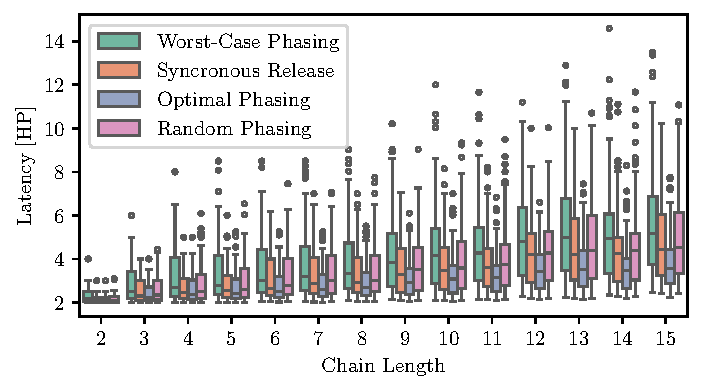
\includegraphics[width=\columnwidth]{plots/LatencyComp.pdf}
	\caption{Comparison of latency under worst-case phasing, synchronous release and optimal phasing. Normalized to the hyperperiod of the chain.}
	\label{fig:latencyComp}
\end{figure}

\begin{figure}
	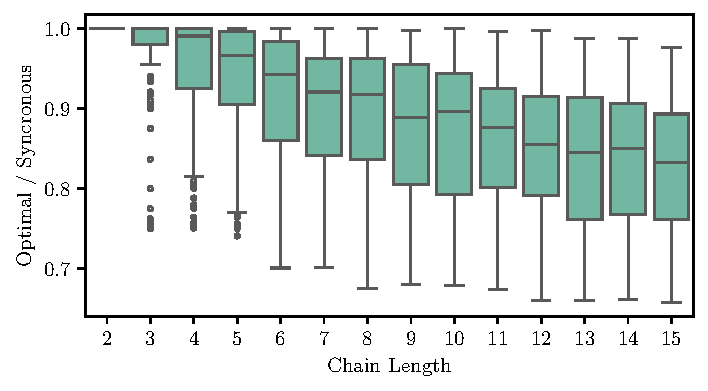
\includegraphics[width=\columnwidth]{plots/LatencyReduction.pdf}
	\caption{Latency reduction with optimal phasing compared to synchronous release.}
	\label{fig:latencyReduction}
\end{figure}

\begin{figure}
	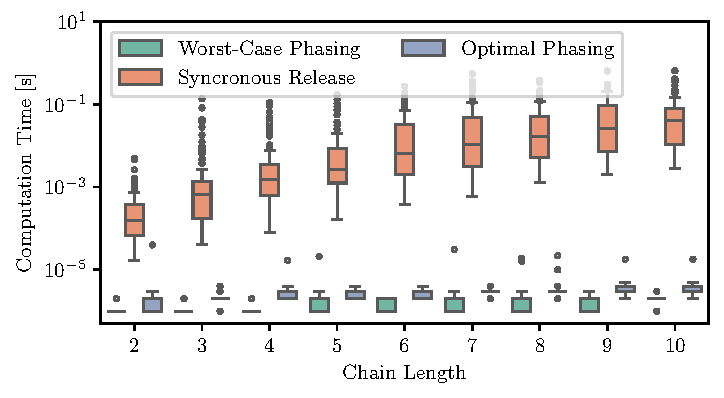
\includegraphics[width=\columnwidth]{plots/AnalysisTimeComp.pdf}
	\caption{Analysis time of the different approaches.}
	\label{fig:analysisTime}
\end{figure}

%\vspace{-0.05in}
\section{Conclusion}
\label{sec:conclusion}


Valuable extensions in future work to 
- constrained deadline task sets
- different communication policies like flexible LET, implicit communication



- arbitrary periods: identify max-harmonic subchains, determine gap-size, try to distribute evenly. (Becomes too complex because then 3 or even more partitioned chains need to be considered for the distribution.)


\appendix
\label{sec:appendix}

We prove Lemma~\ref{lem:repetitive} from page \pageref{lem:repetitive}:

\lemmarepetetive*

\begin{proof}
	\mario{Proof to be adjusted to account for hyperperiod}

	Let $m\geq W_p$.
	In the following we show that $\ell(\pc^p_{m}) 
	= \ell(\pc^p_{m+1})$.
%
	By definition, $\pc^p_m = (\bc_m, \fc_{m+1})$ and $\pc^p_{m+1} = (\bc_{m+1}, \fc_{m+2})$.
	We start by investigating the immediate backward job chains, denoted as 
	$\bc_m = (\tau_1(j_1) \to\dots\to \tau_p(j_p))$ and $\bc_{m+1} = (\tau_1(\tilde{j}_1) \to\dots\to \tau_p({\tilde{j}}_p))$.
	By induction, we show that the jobs of both immediate backward job chains are exactly $T_{\tau_p}$ time units apart, or equivalently
	\begin{equation}\label{eq:induction1}
		j_i + \frac{T_{\tau_p}}{T_{\tau_i}} = \tilde{j}_i
	\end{equation}
	for all $i=p, p{-}1, \dots, 1$.

	\textbf{Base case} ($i=p$):
	By definition of the immediate backward job chains, $j_i = m $ and $\tilde{j}_i = m+1$.
	Hence, $j_i + \frac{T_{\tau_p}}{T_{\tau_i}} = m + \frac{T_{\tau_p}}{T_{\tau_p}} = m+1 = \tilde{j}_i$.

	\textbf{Induction step} ($i \mapsto i-1$):
	By definition of immediate backward job chains, 
	$j_{i-1} = \max \set{\xi \in \Nbb}{ \phi_{\tau_{i-1}} + (\xi+1) \cdot T_{\tau_{i-1}} \leq \phi_{\tau_i} + j_i \cdot T_{\tau_{i}}}$.
	Therefore, $j_{i-1}$ can be formulated as 
	$j_{i-1} = \floor{\frac{\phi_{\tau_i} - \phi_{\tau_{i-1}} + j_i \cdot T_{\tau_i}}{T_{\tau_{i-1}}}} -1$.
	Similarly, $\tilde{j}_{i-1}$ can be written as 
	$\tilde{j}_{i-1} = \floor{\frac{\phi_{\tau_i} - \phi_{\tau_{i-1}} + \tilde{j}_i \cdot T_{\tau_i}}{T_{\tau_{i-1}}}} -1$.
	We know by the induction hypothesis, that $\tilde{j}_i = j_i + \frac{T_{\tau_p}}{T_{\tau_i}}$.
	Therefore, 
	\begin{math}
		\tilde{j}_{i-1} 
		= \floor{\frac{\phi_{\tau_i} - \phi_{\tau_{i-1}} + j_i \cdot T_{\tau_i} + T_{\tau_p}}{T_{\tau_{i-1}}}} -1
		= \floor{\frac{\phi_{\tau_i} - \phi_{\tau_{i-1}} + j_i \cdot T_{\tau_i}}{T_{\tau_{i-1}}} + \frac{T_{\tau_p}}{T_{\tau_i}}} -1
		\overset{\text{(a)}}{=} \floor{\frac{\phi_{\tau_i} - \phi_{\tau_{i-1}} + j_i \cdot T_{\tau_i}}{T_{\tau_{i-1}}}} -1 + \frac{T_{\tau_p}}{T_{\tau_i}}
		= j_{i-1} + \frac{T_{\tau_p}}{T_{\tau_i}}
	\end{math}
	% \begin{align}
	% 	\tilde{j}_{i-1} 
	% 	&= \floor{\frac{\phi_{\tau_i} - \phi_{\tau_{i-1}} + j_i \cdot T_{\tau_i} + T_{\tau_p}}{T_{\tau_{i-1}}}} -1
	% 	= \floor{\frac{\phi_{\tau_i} - \phi_{\tau_{i-1}} + j_i \cdot T_{\tau_i}}{T_{\tau_{i-1}}} + \frac{T_{\tau_p}}{T_{\tau_i}}} -1
	% 	\\& \overset{\text{(a)}}{=} \floor{\frac{\phi_{\tau_i} - \phi_{\tau_{i-1}} + j_i \cdot T_{\tau_i}}{T_{\tau_{i-1}}}} -1 + \frac{T_{\tau_p}}{T_{\tau_i}}
	% 	= j_{i-1} + \frac{T_{\tau_p}}{T_{\tau_i}}
	% \end{align}
	where (a) holds because $\frac{T_{\tau_p}}{T_{\tau_i}} \in \Nbb$ by the max-harmonic property. \qed~Equation~\eqref{eq:induction1}

	In the following we investigate the immediate forward chains, which we denote by
	$\fc_{m+1} = (\tau_p(j'_p) \to\dots\to \tau_n(j'_n))$ and $\fc_{m+2} = (\tau_p(\tilde{j}'_p) \to\dots\to \tau_n({\tilde{j}'}_n))$.
	We show that the jobs of both immediate forward job chains are also exactly $T_{\tau_p}$ time units apart.
	More specifically, we show by induction that 
	\begin{equation}\label{eq:induction2}
		j'_i + \frac{T_{\tau_p}}{T_{\tau_i}} = \tilde{j}'_i
	\end{equation}
	for all $i=p, p{+}1, \dots, n$.
	To achieve this, we additionally show that $j'_i, \tilde{j}'_i > W_i$ during the induction.

	\textbf{Base case} ($i=p$):
	By definition of the immediate forward job chains, $j'_i = m+1 $ and $\tilde{j}'_i = m+2$.
	Hence, $j'_i + \frac{T_{\tau_p}}{T_{\tau_i}} = m +1 + \frac{T_{\tau_p}}{T_{\tau_p}} = m+2 = \tilde{j}'_i$.
	Since $m \geq W_p$ by assumption, we obtain $j'_i = m+1 > W_i$ and $\tilde{j}'_i = m+2 > W_i$.

	\textbf{Induction step} ($i \mapsto i+1$):
	By definition of immediate forward job chains, 
	$j'_{i+1} = \min \set{\xi \in \Nbb}{\phi_{\tau_i} + (j'_i +1) \cdot T_{\tau_i} \leq \phi_{\tau_{i+1}} + \xi \cdot T_{\tau_{i+1}}}$.
	Therefore, $j'_{i+1}$ can be formulated as 
	$j'_{i+1} = \max\setof{\ceiling{\frac{\phi_{\tau_i} - \phi_{\tau_{i+1}} + (j'_i+1) \cdot T_{\tau_i}}{T_{\tau_{i+1}}}} , 0}$.
	
	We start by showing that $j'_{i+1}>W_{i+1}$ by contradiction.
	To that end, assume $j'_{i+1} \leq W_{i+1}$.
	Then, $\re(\tau_{i+1}(j'_{i+1})) \leq \re(\tau_{i+1}(W_{i+1}))$ as well.
	Since $\tau_i(j'_i)$ and $\tau_{i+1}(j'_{i+1})$ are two subsequent jobs in $\fc_{m+1}$, we have $\we(\tau_i(j'_i)) \leq \re(\tau_{i+1}(j'_{i+1}))$.
	Hence, $\we(\tau_i(j'_i)) \leq \re(\tau_{i+1}(W_{i+1}))$ holds.
	Since $W_i$ is the highest integer with $\we(\tau_i(W_i)) \leq \re(\tau_{i+1}(W_{i+1}))$, we obtain $W_i \geq j'_i$ which contradicts the induction hypothesis.

	Since we have shown that $j'_{i+1} > W_{i+1} \geq 0$, we know that $j'_{i+1}>0$.
	Hence, the maximum in $j'_{i+1} = \max\setof{\ceiling{\frac{\phi_{\tau_i} - \phi_{\tau_{i+1}} + (j'_i+1) \cdot T_{\tau_i}}{T_{\tau_{i+1}}}} , 0}$ always returns the first value. 
	That means that $j'_{i+1}$ can be formulated as
	\begin{math}
		j'_{i+1} = \ceiling{\frac{\phi_{\tau_i} - \phi_{\tau_{i+1}} + (j'_i+1) \cdot T_{\tau_i}}{T_{\tau_{i+1}}}}.
	\end{math}
	Similarly, we show that $\tilde{j}'_{i+1} > W_{i+1}$ and that 
	\begin{math}
		\tilde{j}'_{i+1} = \ceiling{\frac{\phi_{\tau_i} - \phi_{\tau_{i+1}} + (\tilde{j}'_i+1) \cdot T_{\tau_i}}{T_{\tau_{i+1}}}}.
	\end{math}
	%
	We utilize the induction hypothesis $\tilde{j}'_i = j'_i + \frac{T_{\tau_p}}{T_{\tau_i}}$ to obtain
	\begin{math}
		\tilde{j}'_{i+1} 
		= \ceiling{\frac{\phi_{\tau_i} - \phi_{\tau_{i+1}} + (j'_i +1) \cdot T_{\tau_i} + T_{\tau_p}}{T_{\tau_{i+1}}}}
		= \ceiling{\frac{\phi_{\tau_i} - \phi_{\tau_{i+1}} + (j'_i +1) \cdot T_{\tau_i}}{T_{\tau_{i+1}}} + \frac{T_{\tau_p}}{T_{\tau_{i+1}}}}
		= \ceiling{\frac{\phi_{\tau_i} - \phi_{\tau_{i+1}} + (j'_i +1) \cdot T_{\tau_i}}{T_{\tau_{i+1}}}} + \frac{T_{\tau_p}}{T_{\tau_{i+1}}}
		= j'_{i+1} + \frac{T_{\tau_p}}{T_{\tau_{i+1}}}
	\end{math}
	% \begin{align}
	% 	\tilde{j}'_{i+1} 
	% 	&= \ceiling{\frac{\phi_{\tau_i} - \phi_{\tau_{i+1}} + (j'_i +1) \cdot T_{\tau_i} + T_{\tau_p}}{T_{\tau_{i+1}}}}
	% 	= \ceiling{\frac{\phi_{\tau_i} - \phi_{\tau_{i+1}} + (j'_i +1) \cdot T_{\tau_i}}{T_{\tau_{i+1}}} + \frac{T_{\tau_p}}{T_{\tau_{i+1}}}}
	% 	\\&
	% 	= \ceiling{\frac{\phi_{\tau_i} - \phi_{\tau_{i+1}} + (j'_i +1) \cdot T_{\tau_i}}{T_{\tau_{i+1}}}} + \frac{T_{\tau_p}}{T_{\tau_{i+1}}}
	% 	= j'_{i+1} + \frac{T_{\tau_p}}{T_{\tau_{i+1}}}
	% \end{align}
	where $\frac{T_{\tau_p}}{T_{\tau_{i+1}}} \in \Nbb$ because the periods are max-harmonic.
	\qed~Equation~\eqref{eq:induction2}

	We conclude that $j_1 + \frac{T_{\tau_p}}{T_{\tau_1}} = \tilde{j}_1$ by Equation~\eqref{eq:induction1} and $j'_n + \frac{T_{\tau_p}}{T_{\tau_n}} = \tilde{j}'_n$ by Equation~\eqref{eq:induction2}.
	Therefore, $\re(\tau_1(j_1)) + T_{\tau_p} = \re(\tau_1(\tilde{j}_1))$ and $\we(\tau_n(j'_n)) + T_{\tau_p} = \we(\tau_n(\tilde{j}'_n))$.
	Hence, we obtain%
	\begin{math}
		\ell(\pc^p_m) = \we(\tau_n(j'_n)) - \re(\tau_1(j_1)) 
		% = \we(\tau_n(j'_n)) + T_{\tau_p}  - \left(\re(\tau_1(j_1)) + T_{\tau_p} \right) 
		= \we(\tau_n(\tilde{j}'_n)) - \re(\tau_1(\tilde{j}_1)) 
		= \ell(\pc^p_{m+1})
	\end{math}
	as desired.
\end{proof}


% bib
\label{last-page}
\clearpage
\bibliographystyle{abbrv}
\bibliography{real-time}
	
\end{document}
